\exercisesheader{}

% 1

\eoce{\qt{Cat weights\label{cat_weights}} The histogram shown below represents 
the weights (in kg) of 47 female and 97 male cats. \footfullcite{cats} \\
\begin{minipage}[c]{0.47\textwidth}
\begin{parts}
\item What fraction of these cats weigh less than 2.5 kg?
\item What fraction of these cats weigh between 2.5 and 2.75 kg?
\item What fraction of these cats weigh between 2.75 and 3.5 kg?
\end{parts} \vspace{27mm}
\end{minipage}
\begin{minipage}[c]{0.05\textwidth}
$\:$ 
\end{minipage}
\begin{minipage}[c]{0.48\textwidth}
\begin{center}
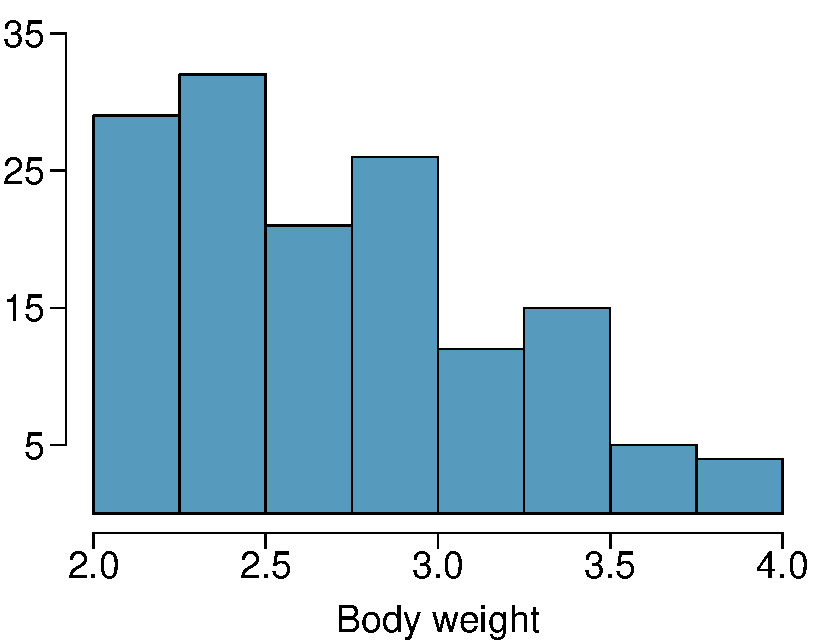
\includegraphics[width=\textwidth]{ch_probability/figures/eoce/cat_weights/cat_weights.pdf}
\end{center}
\end{minipage}
}{}

% 2

\eoce{\qt{Income and gender\label{income_gender}} The relative frequency table 
below displays the distribution of annual total personal income (in 2009 
inflation-adjusted dollars) for a representative sample of 96,420,486 Americans. 
These data come from the American Community Survey for 2005-2009. This sample is 
comprised of 59\% males and 41\% females. \footfullcite{acsIncome2005-2009} \\

\noindent\begin{minipage}[c]{0.60\textwidth}
\begin{parts}
\item Describe the distribution of total personal income.
\item What is the probability that a randomly chosen US resident makes less than 
\$50,000 per year?
\item What is the probability that a randomly chosen US resident makes less than 
\$50,000 per year and is female? Note any assumptions you make.
\item The same data source indicates that 71.8\% of females make less than 
\$50,000 per year. Use this value to determine whether or not the assumption you 
made in part (c) is valid.
\end{parts} 
\end{minipage}
\begin{minipage}[c]{0.4\textwidth}
{\small
\begin{center}
\begin{tabular}{lr}
  \hline
\textit{Income}         & \textit{Total} \\
  \hline
\$1 to \$9,999 or loss  & 2.2\% \\
\$10,000 to \$14,999    & 4.7\% \\
\$15,000 to \$24,999    & 15.8\% \\
\$25,000 to \$34,999    & 18.3\% \\
\$35,000 to \$49,999    & 21.2\% \\
\$50,000 to \$64,999    & 13.9\% \\
\$65,000 to \$74,999    & 5.8\% \\
\$75,000 to \$99,999    & 8.4\% \\
\$100,000 or more       & 9.7\% \\
   \hline
\end{tabular}
\end{center}
}
\end{minipage}
}{}
